\chapter{Implementacja aplikacji}
\thispagestyle{chapterBeginStyle}
\label{rozdzial3}
W tym rozdziale określono szczegóły implementacyjne aplikacji. Scharakteryzowano wykorzystany język programowania oraz użyte biblioteki. Następnie opisano sposób uniemożliwienia dostępu do blokowanych aplikacji. W kolejnej sekcji opisano dokładnie protokół wykorzystywany do komunikacji z MiBandem 3 wraz z sekwencją autentykującą oraz konfiguracyjną. W ostatniej sekcji określono w jaki sposób aplikacja analizuje dane o aktywności użytkownika.

\section{Wykorzystane technologie}
Aplikacja została napisana przy użyciu języka \textbf{Kotlin} w wersji 1.4.31. Język ten, jest tworzony od 2011 roku przez Jetbrains z myślą, by zapewnić przemysłowo silny język obiektowy, który będzie lepszy od Javy ale wciąż będzie z nią w pełni interoperacyjny, aby umożliwić stopniową migrację istniejących już systemów. Głównymi zaletami korzystania z Kotlina w programowaniu na system Android jest zmniejszenie objętości kodu oraz możliwość wykorzystania funkcjonalności języka takich, jak korutyny, funkcje rozrzerzeń czy lambdy w istniejących bibliotekach Androida. Kod Kotlina jest także bardziej czytelny niż Javy, co prowadzi do zmniejszonej liczby błędów. 
\newline\newline
\indent Do implementacji bazy danych wykorzystano bibliotekę \textbf{Room}, tworzącą warstwę abstrakcji nad SQLite, by zapewnić płynny dostęp do bazy, zachowując pełną moc SQLite. Biblioteka ta pozwala między innymi zmniejszyć ilość powtarzalnego, skłonnego do generowania błędów kodu poprzez stosowanie anotacji oraz weryfikować zapytania SQL w czasie kompilacji. Aby zapewnić bezpieczeństwo bazy danych została ona zaszyfrowana przy użyciu biblioteki \textbf{SQLCipher}.
\newline\newline
\indent Do jeszcze większej optymalizacji kodu wykorzystano bibliotekę \textbf{Hilt}, która odpowiada za wstrzykiwanie zależności do klas. W przeciwieństwie do manualnego konstruowania klas wraz z ich zależnościami oraz wykorzystywaniu dodatkowych obiektów do zarządzania nimi, Hilt generuje je sam na podstawie określonych anotacji, a także zapewnia poprawne zarządzanie ich cyklem życia. Dzięki temu przy mniejszej ilości kodu można uzyskać lepszą wydajność w czasie działania aplikacji oraz zmiejszenie liczby błędów podczas kompilacji.
\newline\newline
\indent Do implementacji komunikacji z MiBandem została wykorzystana biblioteka \textbf{RxJava}, pozwalająca wykorzystać możliwości programowania reaktywnego, czyli paradygmatu programowania polegającego na przetwarzaniu strumieni danych i propagowaniu ich zmian, w aplikacjach na system Android. Przepływ danych pomiędzy aplikacją a opaską został opakowany w obiekty typu \textit{Observable}, co pozwoliło dokładnie monitorować stan wysyłanych danych oraz asynchronicznie oczekiwać odpowiedzi na poszczególne operacje.
\newline\newline
\indent Aby usprawnienić wydajność aplikacji wszystkie operacje zapisu do bazy danych oraz komunikacja z opaską są wykonywane w korutynach zoptymalizowanych pod operacje wejścia/wyjścia, dzięki czemu główny wątek aplikacji zostaje odciążony. Wykorzystano również \textbf{Data Binding}, aby uprościć odniesienia do elementów UI w kodzie aplikacji, co pozwala zwiększyć odporność na wycieki pamięci oraz wydajność. 

\section{Blokada dostępu do aplikacji}
Skuteczny sposób uniemożliwienia dostępu do aplikacji jest jedną z kluczowych części projektowanego systemu. Schemat blokady zaprezentowany w pracy opiera się na monitorowaniu aplikacji na pierwszym planie systemu Android. Aby dostać się do tych informacji wykorzystano usługę \textit{Usage Stats}, która zawiera statystyki korzystania z zainstalowanych aplikacji oraz zdarzenia takie, jak zablokowanie ekranu czy wyświetlenie aktywności danej aplikacji na ekranie. Proponowany system blokady pobiera zdarzenia z ostatnich 5 sekund, a następnie poszukuje w nich typu ``MOVE\_TO\_FOREGROUND''. Jeśli takie zdarzenie zostanie odnalezione, a aplikacja, która zainicjowała je, jest na liście aplikacji do zablokowania, następuje przejście do aktywności zawierającej pole do wpisania hasła. W przeciwnym razie system nie reaguje. Jeśli wprowadzone hasło było poprawne, usługa blokująca zostaje zatrzymana i aplikacja nawiązuje próbę połączenia się z opaską. Poniżej przedstawiono zarys algorytmu blokującego w pseudokodzie.
\newline

\begin{algorithm}[H]
    \DontPrintSemicolon
    \SetAlgorithmName{Algorytm}{algorytm}{Lista algorytmów}
    \SetKwInput{KwData}{Dane}%
    \SetKwInput{KwResult}{Wynik}%
    \SetAlgoLined
    \caption{Blokowanie dostępu do wybranych aplikacji} 
    \BlankLine
    \KwData{Lista zablokowanych aplikacji $BA$}
    \BlankLine
    \Begin{
        \While{blokada jest aktywna}{
            $events \gets $ zdarzenia z \textit{Usage Stats} z ostatnich 5 sekund \;
            \While{$events$.hasNext()}{
                $event \gets events$.next() \;
                \If{$event ==$ ``MOVE\_TO\_FOREGROUND'' $\land$ $event$.isIn($BA$)}{
                    Uruchom aktywność odpowiedzialną za wpisywanie hasła \;
                }
            }
            Poczekaj 5 sekund \;
        }
    }
\end{algorithm}

\section{Komunikacja z MiBand 3}
W projektowanym systemie główną rolę gra inteligentna opaska. Komunikuje się ona ze smartfonem przy użyciu Bluetooth Low Energy protokołem ATT korzystając z GATT. BLE w porównaniu do klasycznego połączenia Bluetooth wykorzystuje znacznie niższe zasoby energii zachowując podobny zasięg, dzięki czemu znalazło szerokie zastosowanie w urządzeniach peryferyjnych. W poniższych podrozdziałach opisano pokrótce pojęcia ATT i GATT oraz dokładnie przedstawiono zaimplementowany protokół komunikacji z opaską MiBand 3.
\subsection{ATT}
Protokół Attribute umożliwia urządzeniu, określonemu jako \textit{serwer}, odsłonić zbiór atrybutów i powiązanych z nimi wartości urządzeniu równorzędnemu, określonemu jako \textit{klient}. Atrybuty odsłonięte przez serwer mogą być odkryte, odczytane bądź nadpisane przez klienta, a także mogą być rozgłaszane przez serwer w ramach powiadomienia lub zasygnalizowania. Atrybut jest dyskretną wartością o trzech właściwościach powiązanych ze sobą:
\begin{itemize}
    \item typie,
    \item uchwycie,
    \item zestawie pozwoleń, które są zdefiniowane przez specyfikację wyższej warstwy wykorzystującą dany atrybut.
\end{itemize}
Typ atrybutu określa, co reprezentuje dany atrybut poprzez UUID (Universally Unique Identifier), ktore może zostać utworzone przez każdego, a następnie zostać opublikowane. Pozwala to rozpoznać atrybut niezależnie od nadanego mu przez serwer uchwytu. Uchwyt atrybutu jest unikalną, niezerową, 16-bitową wartością, która jednoznacznie identyfikuje dany atrybut w obrębie serwera, pozwalając klientowi odnieść się do niego podczas operacji odczytu oraz zapisu. Pozwolenia mogą być nadane atrybutowi w celu ograniczenia klientowi dostępu do zapisu lub odczytu.
\newline\newline
\indent Urządzenie może jednocześnie implementować zarówno rolę serwera jak i klienta oraz obie role mogą funkcjonować współbieżnie oraz komunikować się między sobą. Na każdym urządzeniu Bluetooth może znajdować się maksymalnie jedna instancja serwera.
\newline\newline
\indent Wszystkie prośby protokołu Attribute są przesyłane poprzez \textit{nosiciela ATT}. Między urządzeniami może być wielu nosicieli, gdzie każdy z nich korzysta z osobnego kanału L2CAP oraz może mieć inną konfigurację. W przypadku BLE, wykorzystywany jest pojedynczy nosiciel ATT, który używa stałego kanału dostępnego od ustanowienia połączenia ACL. Można jednak skonfigurować dodatkowych nosicieli używając L2CAP. Więcej informacji na temat protokołu ATT można znaleźć w \cite{BT-Corev5.2}. 

\subsection{GATT}
Profil Generic Attribute (GATT) definiuje framework wykorzystujący protokół Attribute, określający procedury i formaty danych znajdujących się wewnątrz profilu. Zdefiniowane procedury obejmują odkrywanie, odczyt, zapis, powiadamianie oraz sygnalizację. Profil ten został zaprojektowany do wykorzystania przez aplikacje bądź inny profil, aby umożliwić klientowi komunikację z serwerem poprzez opakowanie protokołu ATT w bardziej przystępną formę.
\newline\newline
\indent Profil GATT określa strukturę, w której odbywa się wymiana danych. Najwyższym poziomem jest profil zawierający liczne \textit{usługi} będące zbiorem danych oraz przypisanych im zachowań niezbędnych do zapewnienia określonej funkcji. Usługi składają się z \textit{charakterystyk}, z których każda zawiera określoną wartość oraz opcjonalne informacje na jej temat. Usługi oraz charakterystyki wraz ze swoimi komponentami zawierają dane profilu, które są przechowywane w Atrybutach na serwerze. Dzięki wykorzystaniu określonej struktury danych przez GATT możliwe jest przeglądanie dostępnych Usług oraz Charakterystyk, nawet gdy klient nie jest wyspecjalizowany pod dany serwer. Więcej informacji na temat GATT można znaleźć w \cite{BT-Corev5.2}.

\subsection{Inżynieria wsteczna protokołu komunikacji opaski}
Zważywszy na to, iż protokół komunikacji opaski MiBand 3 nie jest jawny, konieczne było zastosowanie inżynierii wstecznej w celu identyfikacji usług oraz charakterystyk wraz z ich funkcjonalnością. Dane do analizy uzyskano przechwytując pakiety ATT między opaską a aplikacją Gadgetbridge \cite{Gadgetbridge} przy użyciu sniffera Wireshark \cite{Wireshark}. Korzystając z faktu, że Gadgetbridge jest open-source możliwe było użycie kodu źródłowego aplikacji do interpretacji zaobserwowanych przesyłanych wartości. Na poniższych grafikach przedstawiono dwa przykładowe pakiety przechwycone w czasie analizy protokołu. 
\begin{figure}[H]
    \begin{center}
        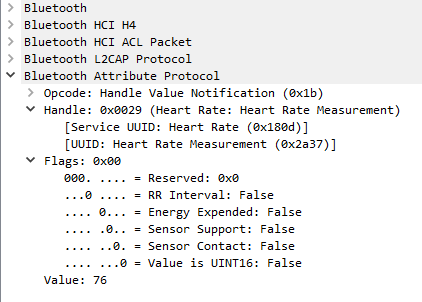
\includegraphics[width=0.36\textwidth]{HRPacket.png}
    \end{center}
    \caption{{\color{dgray}Przechwycony pakiet zawierający wartość akcji serca.}} \label{hrPacket}
\end{figure}
\begin{figure}[H]
    \begin{center}
        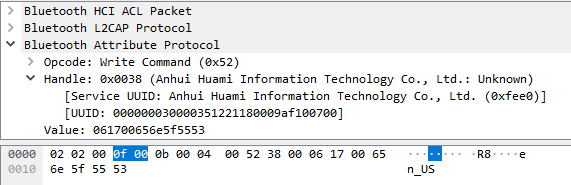
\includegraphics[width=0.60\textwidth]{SetLanguageATTPacket.png}
    \end{center}
    \caption{{\color{dgray}Przechwycony pakiet zawierający konfigurację języka w opasce na angielski.}} \label{langPacket}
\end{figure}
\subsection{Wykorzystane usługi i charakterystyki}
Na podstawie przeprowadzonych analiz komunikacji, wyszczególniono poniższe usługi i charakterystyki, które posłużyły do realizacji funkcjonalności tworzonej aplikacji.

\subsubsection{Usługa 0000fee0-0000-1000-8000-00805f9b34fb}
Jest to usługa odpowiadająca w głównej mierze za podstawowe funkcjonalności opaski MiBand 3. Pozwala zmodyfikować ustawienia urządzenia, zapisać informacje o użytkowniku oraz odczytać dane o stanie baterii i aktywności użytkownika. Jest to najczęściej wykorzystywana usługa w aplikacji.

\begin{table}[H]
    \bgroup
    \def\arraystretch{1.5}%
    \begin{tabular}{|ll|}
    \hline
    \textbf{Charakterystyka}                      & \textbf{Opis}                                                                                                                \\ \hline
    \textbf{00000003-0000-3512-2118-0009af100700} & \begin{tabular}[c]{@{}l@{}}Charakterystyka pozwalająca na konfigurację ustawień \\ opaski.\end{tabular}                      \\
    \textbf{00000006-0000-3512-2118-0009af100700} & \begin{tabular}[c]{@{}l@{}}Charakterystyka zawierająca informacje o stanie baterii \\ opaski.\end{tabular}                   \\
    \textbf{00000007-0000-3512-2118-0009af100700} & \begin{tabular}[c]{@{}l@{}}Charakterystyka przechowująca liczbę wykonanych kroków \\ danego dnia.\end{tabular}               \\
    \textbf{00000008-0000-3512-2118-0009af100700} & Charakterystyka zawierająca dane użytkownika.                                                                                \\
    \textbf{00000010-0000-3512-2118-0009af100700} & \begin{tabular}[c]{@{}l@{}}Charakterystyka zawierająca informacje na temat zdarzeń \\ wykrywanych przez opaskę.\end{tabular} \\
    \textbf{00002a2b-0000-1000-8000-00805f9b34fb} & Charakterystyka przechowująca aktualną datę i godzinę,                                                                       \\ \hline
    \end{tabular}
    \egroup
    \caption{{\color{dgray}Wykorzystane charakterystyki z usługi 0000fee0-0000-1000-8000-00805f9b34fb.}} \label{miliservice}
\end{table}

\subsubsection{Usługa 0000fee1-0000-1000-8000-00805f9b34fb}
Jest to usługa zawierająca przede wszystkim charakterystykę wykorzystywaną w procesie autentykacji połączenia oraz parowania. W usłudze tej znajduje się też sporo niezidentyfikowanych charakterystyk, które nie są wymagane do działania aplikacji. Dlatego więc zostały pominięte.
\begin{table}[H]
    \bgroup
    \def\arraystretch{1.5}%
    \begin{tabular}{|ll|}
    \hline
    \textbf{Charakterystyka}                      & \textbf{Opis}                                                                                                                \\ \hline
    \textbf{00000009-0000-3512-2118-0009af100700} & \begin{tabular}[c]{@{}l@{}}Charakterystyka wykorzystywana do autentykacji  \\ połączenia między opaską a klientem\end{tabular} \\ \hline
    \end{tabular}
    \egroup
    \caption{{\color{dgray}Wykorzystane charakterystyki z usługi 0000fee1-0000-1000-8000-00805f9b34fb.}} \label{miband2service}
\end{table}

\subsubsection{Usługa 0000180d-0000-1000-8000-00805f9b34fb}
Jest to usługa zdefiniowana przez Bluetooth Special Interest Group odpowiadająca za komunikację między sensorem akcji serca a innym klientem GATT. Za jej pomocą można uzyskać informację o pulsie użytkownika oraz skonfigurować automatyczne pomiary. 

\begin{table}[H]
    \bgroup
    \def\arraystretch{1.5}%
    \begin{tabular}{|ll|}
    \hline
    \textbf{Charakterystyka}                      & \textbf{Opis}                                                                                                              \\ \hline
    \textbf{00002a37-0000-1000-8000-00805f9b34fb} & \begin{tabular}[c]{@{}l@{}}Charakterystyka wykorzystywana do odczytu aktualnej \\ wartości pulsu użytkownika.\end{tabular} \\
    \textbf{00002a39-0000-1000-8000-00805f9b34fb} & \begin{tabular}[c]{@{}l@{}}Charakterystyka odpowiedzialna za konfigurację sensora \\ akcji serca w opasce.\end{tabular}    \\ \hline
    \end{tabular}
    \egroup
    \caption{{\color{dgray}Wykorzystane charakterystyki z usługi 0000180d-0000-1000-8000-00805f9b34fb.}} \label{heartrateservice}
\end{table}

\subsubsection{Usługa 0000180a-0000-1000-8000-00805f9b34fb}
Jest to usługa również zdefiniowana przez Bluetooth Special Interest Group. Odpowiada za dostarczenie informacji o urządzeniu. W tym wypadku jest to informacja o numerze seryjnym opaski oraz wersjach sprzętu i oprogramowania.

\begin{table}[H]
    \bgroup
    \def\arraystretch{1.5}%
    \begin{tabular}{|ll|}
    \hline
    \textbf{Charakterystyka}                      & \textbf{Opis}                                                                                                      \\ \hline
    \textbf{00002a25-0000-1000-8000-00805f9b34fb} & \begin{tabular}[c]{@{}l@{}}Charakterystyka wykorzystywana do odczytu numeru \\ seryjnego opaski.\end{tabular}      \\
    \textbf{00002a27-0000-1000-8000-00805f9b34fb} & \begin{tabular}[c]{@{}l@{}}Charakterystyka wykorzystywana do odczytu wersji \\ sprzętowej opaski.\end{tabular}        \\
    \textbf{00002a28-0000-1000-8000-00805f9b34fb} & \begin{tabular}[c]{@{}l@{}}Charakterystyka wykorzystywana do odczytu wersji \\ oprogramowania opaski.\end{tabular} \\ \hline
    \end{tabular}
    \egroup
    \caption{{\color{dgray}Wykorzystane charakterystyki z usługi 0000180a-0000-1000-8000-00805f9b34fb.}} \label{deviceservice}
\end{table}

\subsection{Autentykacja połączenia}
Aby konfigurować oraz odczytywać informacje o aktywności z MiBanda wymagana jest prosta autoryzacja. W przeciwnym razie ma dostępu do większości charakterystyk urządzenia, a połączenie zostanie zerwane po 30 sekundach. Sekwencja autentykacyjna wygląda w następujący sposób. Najpierw do opaski należy wysłać klucz, który zostanie wykorzystany do autentykacji połączenia. Wykonuje się to przy pierwszym połączeniu z urządzeniem. Następnie wysyłana jest prośba do MiBanda o podanie losowej liczby. Po jej otrzymaniu należy zaszyfrować ją algorytmem AES korzystając z klucza podanego przy parowaniu opaski, odesłać i przesłać aktualną datę do odpowiedniej charakterystyki. Po otrzymaniu potwierdzenia połączenie jest zatwierdzone i można przejść do sekwencji konfigurującej. Aktualna data przesyłana jest jako tablica bajtów. Dostęp do odpwiednich wartości można uzyskać przez przesunięcie bitowe i maskowanie odpowiednich bitów, co przedstawiono dokładnie na grafice poniżej:
\begin{figure}[H]
    \begin{center}
        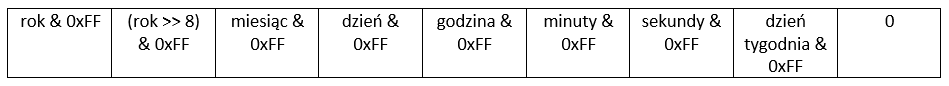
\includegraphics[width=0.90\textwidth]{DateByteArray.png}
    \end{center}
    \caption{{\color{dgray}Struktura tablicy bajtów zawierającej aktualną datę.}} \label{dateByteArray}
\end{figure}

\begin{algorithm}[H]
    \DontPrintSemicolon
    \SetAlgoLined
    \SetAlgorithmName{Algorytm}{algorytm}{Lista algorytmów}
    \SetKwInput{KwData}{Dane}%
    \SetKwInput{KwResult}{Wynik}%
    \caption{Parowanie z MiBandem 3} 
    \BlankLine
    \KwData{Tablica bajtów zawierająca klucz wykorzystywany do szyfrowania $K$, Zmienna logiczna $pair$ mówiąca, czy urządzenie jest sparowane}
    \BlankLine
    \Begin{
        $authorisationChar \gets 00000009-0000-3512-2118-0009af100700$\;
        Włącz powiadomienia na $authorisationChar$\;
        \If{$pair$}{
            Wyślij do $authorisationChar \longrightarrow ByteArray(0x01, 0x00) + K $\;
            \If{Otrzymano $odpowiedz \gets ByteArray(0x10, 0x01, 0x01)$}{
                Przejdź do autentykacji \;
            }
        }
    }
\end{algorithm}
\quad\newline\newline
\begin{algorithm}[H]
    \DontPrintSemicolon
    \SetAlgoLined
    \SetAlgorithmName{Algorytm}{algorytm}{Lista algorytmów}
    \SetKwInput{KwData}{Dane}%
    \SetKwInput{KwResult}{Wynik}%
    \caption{Autentykacja z MiBandem 3} 
    \BlankLine
    \KwData{Tablica bajtów zawierająca klucz wykorzystywany do szyfrowania $K$}
    \BlankLine
    \Begin{
        $authorisationChar \gets 00000009-0000-3512-2118-0009af100700$\;
        $timeChar \gets 00002a2b-0000-1000-8000-00805f9b34fb$\;
        Włącz powiadomienia na $authorisationChar$\;
        Wyślij do $authorisationChar \longrightarrow ByteArray(0x02, 0x00)$\;
        \If{Otrzymano $odpowiedz \gets ByteArray(0x10, 0x02, 0x01, \dots)$}{
            $numToEncrypt \gets odpowiedz \left[ 3:19 \right]$ \;
            Wyślij do $authorisationChar \longrightarrow ByteArray(0x03, 0x00) + AES(K, numToEncrypt)$ \;
            Wyślij do $timeChar$ aktualną datę\;
        }
        \If{Otrzymano $odpowiedz \gets ByteArray(0x10, 0x03, 0x01, \dots)$}{
            Przejdź do konfiguracji\;
        }
    }
\end{algorithm}

\subsection{Sekwencja konfigurująca}
Po udanej autoryzacji połączenia należy skonfigurować działanie opaski. Odbywa się to za pomocą sekwencji operacji zapisu, głównie do charakterystyki o UUID równym ``00000003-0000-3512-2118-0009af100700'' oraz włączeniu powiadamiania na odpowiednich charakterystykach. Po skonfigurowaniu urządzenie będzie automatycznie przesyłać odpowiednie dane o aktywności w najmniejszych możliwych odstępach czasu. Na poniższych grafikach przedstawiono struktury tablic bajtów wysyłanych danych, które były zbyt obszerne, aby przedstawić je w pseudokodzie. 
\begin{figure}[H]
    \begin{center}
        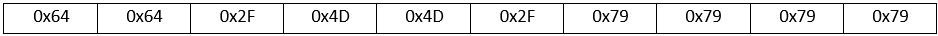
\includegraphics[width=0.90\textwidth]{DateFormatBA.png}
    \end{center}
    \caption{{\color{dgray}Tablica bajtów zawierająca format wyświetlanej w opasce daty - dd/MM/yyyy.}} \label{dateFormat}
\end{figure}
\begin{figure}[H]
    \begin{center}
        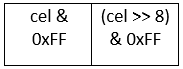
\includegraphics[width=0.20\textwidth]{FitnessGoalBA.png}
    \end{center}
    \caption{{\color{dgray}Tablica bajtów zawierająca cel aktywności - liczbę kroków do wykonania dziennie.}} \label{fitnessGoal}
\end{figure}
\begin{figure}[H]
    \begin{center}
        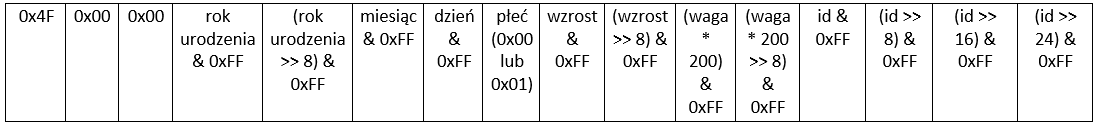
\includegraphics[width=0.90\textwidth]{UserInfoBA.png}
    \end{center}
    \caption{{\color{dgray}Tablica bajtów zawierająca informacje o użytkowniku.}} \label{userInfo}
\end{figure}

\begin{algorithm}[H]
    \DontPrintSemicolon
    \SetAlgoLined
    \SetAlgorithmName{Algorytm}{algorytm}{Lista algorytmów}
    \SetKwInput{KwData}{Dane}%
    \SetKwInput{KwResult}{Wynik}%
    \caption{Konfiguracja MiBanda 3 - Część 1} 
    \BlankLine
    \Begin{
        $settingsChar \gets 00000003-0000-3512-2118-0009af100700$\;
        $batteryChar \gets 00000006-0000-3512-2118-0009af100700$\;
        $eventsChar \gets 00000010-0000-3512-2118-0009af100700$\;
        $userChar \gets 00000008-0000-3512-2118-0009af100700$\;
        $hrControlChar \gets 00002a39-0000-1000-8000-00805f9b34fb$\;
        $hrChar \gets 00002a37-0000-1000-8000-00805f9b34fb$\;
        $stepsChar \gets 00000007-0000-3512-2118-0009af100700$\;
        $serialNumChar \gets 00002a25-0000-1000-8000-00805f9b34fb$\;
        $hardwareChar \gets 00002a27-0000-1000-8000-00805f9b34fb$\;
        $softwareChar \gets 00002a28-0000-1000-8000-00805f9b34fb$\;
        \;
        Włącz powiadomienia na $settingsChar, batteryChar$ oraz $eventsChar$\;
        Odczytaj wartość z $serialNumChar, hardwareChar, softwareChar$ oraz $batteryChar$\;
        Ustaw język angielski wysyłając $ByteArray(0x06, 0x17, 0x00, 0x65, 0x6e, 0x5f, 0x55, 0x53)$ do $settingsChar$ \;
        Wyłącz odblokowywanie ekranu w opasce wysyłając $ByteArray(0x06, 0x16, 0x00, 0x00)$ do $settingsChar$\;
        Wyłącz tryb nocny wysyłając $ByteArray(0x1a, 0x00)$ do $settingsChar$\;
        Ustaw format daty wysyłając $ByteArray(0x06, 0x1e, 0x00)+ format$ do $settingsChar$, gdzie $format$ to opisany powyżej przetworzony łańcuch znaków\;
        Ustaw format wyświetlanej daty wysyłając $ByteArray(0x06, 0x0a, 0x00, 0x03)$ do $settingsChar$\;
        Ustaw 24-godzinny zegar wysyłając $ByteArray(0x06, 0x02, 0x00, 0x01)$ do $settingsChar$\;
        Ustaw przykładowe dane o użytkowniku wysyłając $userInfo$ do $settingsChar$, gdzie $userInfo$ to przetworzone dane o użytkowniku opisane powyżej\;
        Ustaw jednostki metryczne wysyłając $ByteArray(0x06, 0x03, 0x00, 0x00)$ do $settingsChar$\;
        Włącz powiadomienia na $userChar$\;
        Ustaw lokalizację noszenia opaski na lewą rękę wysyłając $ByteArray(0x20, 0x00, 0x00, 0x02)$ do $userChar$\;
        Ustaw cel fitness wysyłając $ByteArray(0x10, 0x00, 0x00, x[0], x[1], 0x00, 0x00)$ do $userChar$, gdzie $x$ to przetworzona wartość celu\;
        Ustaw elementy menu opaski wysyłając $ByteArray(0x0a, 0x7f, 0x30, 0x00, 0x01, 0x02, 0x03, 0x04, 0x05, 0x06, 0x07, 0x08)$ do $settingsChar$\;
        Wyłącz w opasce tryb ``Nie przeszkadzać'' wysyłając $ByteArray(0x09, 0x82)$ do $settingsChar$\;
    }
\end{algorithm}
\quad\newline\newline
\begin{algorithm}[H]
    \DontPrintSemicolon
    \SetAlgoLined
    \SetAlgorithmName{Algorytm}{algorytm}{Lista algorytmów}
    \SetKwInput{KwData}{Dane}%
    \SetKwInput{KwResult}{Wynik}%
    \caption{Konfiguracja MiBanda 3 - Część 2} 
    \BlankLine
    \Begin{
        Wyłącz gest obrotu nadgarstka do zmiany pozycji w menu wysyłając $ByteArray(0x06, 0x0d, 0x00, 0x00)$ do $settingsChar$\;
        Wyłącz gest podniesienia nadgarstka do włączenia ekranu opaski wysyłając $ByteArray(0x06, 0x05, 0x00, 0x00)$ do $settingsChar$\;
        Włącz wyświetlanie ID dzwoniącego w opasce wysyłając $ByteArray(0x06, 0x10, 0x00, 0x00, 0x01)$ do $settingsChar$\;
        Wyłącz powiadomienia o celu fitness wysyłając $ByteArray(0x06, 0x06, 0x00, 0x00)$ do $settingsChar$\;
        Wyłącz powiadomienia o nieaktywności wysyłając $ByteArray(0x08, 0x00, 0x3c, 0x00, 0x04, 0x00, 0x15, 0x00, 0x00, 0x00, 0x00, 0x00)$ do $settingsChar$\;
        Włącz wspomaganie detekcji snu przez pomiar pulsu wysyłając $ByteArray(0x15, 0x00, 0x01)$ do $hrControlChar$\;
        Włącz powiadomienie o utracie połączenia wysyłając $ByteArray(0x06, 0x0c, 0x00, 0x01, 0x00, 0x00, 0x00, 0x00)$ do $settingsChar$\;
        Włącz powiadomienie o nawiązaniu połączenia wysyłając $ByteArray(0x06, 0x01, 0x00, 0x01)$ do $settingsChar$\;
        Ustaw interwał automatycznego pomiaru pulsu na minimalny wysyłając $ByteArray(0x14, 0x01)$  do $hrControlChar$\;
        Poproś o alarmy wysyłając $0x0d$ do $settingsChar$\;
        Włącz powiadomienia na $hrChar$ oraz $stepsChar$\;
    }
\end{algorithm}

\section{Analiza rejestrowanych danych o aktywności}
Aby proponowany system działał poprawnie niezbędna jest analiza gromadzonych przez opaskę oraz sensor kroków danych. Aplikacja rozróżnia 4 typy aktywności:
\begin{itemize}
    \item puls,
    \item kroki rejestrowane w opasce,
    \item kroki rejestrowane w telefonie,
    \item oraz inne zdarzenia.
\end{itemize}
Próbki pulsu oraz kroków są przechowywane w bazie danych w celu analizy. Natomiast wykrycie zdarzeń innego typu samo w sobie jest przesłanką do zablokowania systemu, więc nie ma potrzeby ich przechowywania. W poniższych akapitach opisano sposoby monitorowania zarejestrowanych próbek i zdarzeń oraz sytuacje, w których jest uruchamiana blokada.
\newline\newline
\indent Dane o akcji serca są analizowane w następujący sposób. Każda nadchodząca próbka z pomiarem równym 0 oraz brak zarejestrowania żadnej próbki w ciągu 90 sekund, świadczy o tym, że opaska została zdjęta i jest to przesłanka do blokady systemu. Z testów przeprowadzonych podczas rozwoju aplikacji wynikło, że monitorowanie tych czynników z wykorzystaniem podanych wartości jest ważne dla poprawnego określenia, czy opaska znajduje się na ręce, gdyż MiBand 3 rejestruje zdarzenia z opóźnieniem, więc odpowiednie zdarzenie o zdjęciu opaski nadchodziło po kilku minutach, co nie zapewnia wystarczającego bezpieczeństwa. Z kolei łączenie z opaską również jest obarczone sporym opóźnieniem, dlatego czasem w ciągu 60 sekund (najkrótszy możliwy okres pomiędzy automatycznymi pomiarami pulsu) od włączenia systemu monitorującego nie rejestrowano żadnej próbki pulsu. Z tego powodu okres pomiędzy pobieraniem próbek z bazy musiał zostać zwiększony do 90 sekund.
\newline\newline
\indent Dane o krokach są analizowane na podstawie różnic w tempie wzrostu między próbkami z opaski oraz smartfona. Co 90 sekund system pobiera próbki z ostatnich 90 sekund. Jeśli dla jednego ze źródeł nie zarejestrowano nowych próbek, system pobiera datę ostatniego pomiaru z tego źródła, a następnie dopisuje do listy próbek z drugiego źródła próbki starsze niż 90 sekund i młodsze od ostatniej próbki z pierwszego źródła. Krok ten został podjęty w celu wykrycia sytuacji, gdzie tylko jedno urządzenie porusza się, jednak na tyle wolno, że system myślałby, że tempa wzrostu pomiędzy tymi źródłami są akceptowalne. Tempo wzrostu jest określone jako amplituda wartości kroków z pobranych wcześniej próbek, biorąc poprawkę na możliwość pobrania próbek z okresu, gdy zmienia się data, co powoduje rozpoczęcie liczenia kroków od 0. Akceptowalna wartość amplitudy wynosi $\leq 30$. Jest to uwarunkowane tym, że przy niższych wartościach system mógłby aktywować się przy poruszaniu się wraz z telefonem, a przy wyższych system nie zareagowałby w wystarczającym stopniu na podejrzane sytuacje.
\newline\newline
\indent Oprócz analizy próbek aktywności system reaguje też na wykrywane zdarzenia. System rejestruje zdjęcie opaski, zaśnięcie oraz utratę połączenia. W przypadku dwóch pierwszych sytuacji, blokada jest uruchamiana natychmiastowo. Natomiast w przypadku utraty połączenia podejmowane są dwie próby ponownego połączenia. Jeśli nie uda się nawiązać ponownie połączenia uruchamiana jest blokada.